\documentclass[red,slidestop,notes,compress,mathserif]{beamer}

%\usepackage{beamerthemesplit}
\setbeamertemplate{navigation symbols}{}
\setbeamertemplate{note page}[plain]

\usetheme{Boadilla}
\usepackage{wasysym}
\usefonttheme{professionalfonts} % using non standard fonts for beamer
\usefonttheme{serif} % default family is serif
\usepackage{fontspec}

\usepackage{fontspec}
%\newfontfamily\greekfont[Mapping=tex-text]{DejaVu Serif}
%\setmainfont{Liberation Serif}


\title[CloudDP '15, Bordeaux]{V4VSockets: low-overhead intra-node communication in Xen.} 
\author[A. Nanos]{Anastassios Nanos, Stefanos Gerangelos, Ioanna Alifieraki, Nectarios Koziris}
\date{Apr. 21st, 2015}
\logo{\includegraphics[scale=0.05]{figures/ntua_logo.pdf}\includegraphics[scale=0.16]{figures/cslab_logo.pdf}}

\institute[CSLab, NTUA]{High-Performance Systems and Interconnects (HPSI),\\
Computing Systems Lab\\National Technical University of Athens\\
Github: \url{http://github.com/HPSI}\\
WWW: \url{http://cslab.ece.ntua.gr/research/}\\
\includegraphics[width=1.5cm]{figures/ntua_logo.pdf}
\includegraphics[width=3.5cm]{figures/cslab_logo.pdf}\\
%\includegraphics[angle=-90,width=4.0cm]{figs/hrakleitos.pdf}\\
}


\newcommand{\ta}{\insertframenumber}

%\AtBeginSubsection[]
%{
%  \begin{frame}
%  \frametitle{Overview}
%  \tableofcontents[currentsection,currentsubsection]
%  \end{frame}
%}
\begin{document}



\frame{\titlepage}

  \begin{frame}
  \frametitle{Overview}
  \tableofcontents[]%[currentsection,currentsubsection]
  \end{frame}
\section*{Introduction}

\begin{frame}
\frametitle{Introduction}
\begin{block}{Cloud computing}
\begin{itemize}
\item application oriented
\item fast, ease-of-use
\end{itemize}
\end{block}
\begin{block}{Consolidation}
\begin{itemize}
\item $\frac{vCPU}{physical cores}$ $>>$ 1
\item multi/many--cores  
\end{itemize}
\end{block}
%\pause
\begin{block}{}
The number of co-located VMs is drastically increasing
\end{block}
%\pause
%\end{frame}

%\pause
\end{frame}

\begin{frame}
\frametitle{Introduction}
\begin{block}{Applications}
\begin{itemize}
\item stand-alone (flexibility)
\item distributed (elasticity)
\item relatively recent trend: network flows (SDN/NFV)
\end{itemize}
The need for intra-node communication increases.
\end{block}
\pause
\begin{block}{Design and implement V4VSockets:}
\begin{itemize}
\item efficient message exchange (almost one order of magnitude better than generic approaches)
\item isolation
\item API compatible (Sockets)
\end{itemize}
\end{block}

\end{frame}


\section{Communication in Virtual Environments}

\subsection{Basic Concepts}

\begin{frame}
\frametitle{Xen - Architecture}
\begin{itemize}
\item hypervisor \& privileged VM (driver domain) to access hardware
\end{itemize}
\begin{figure}
\center
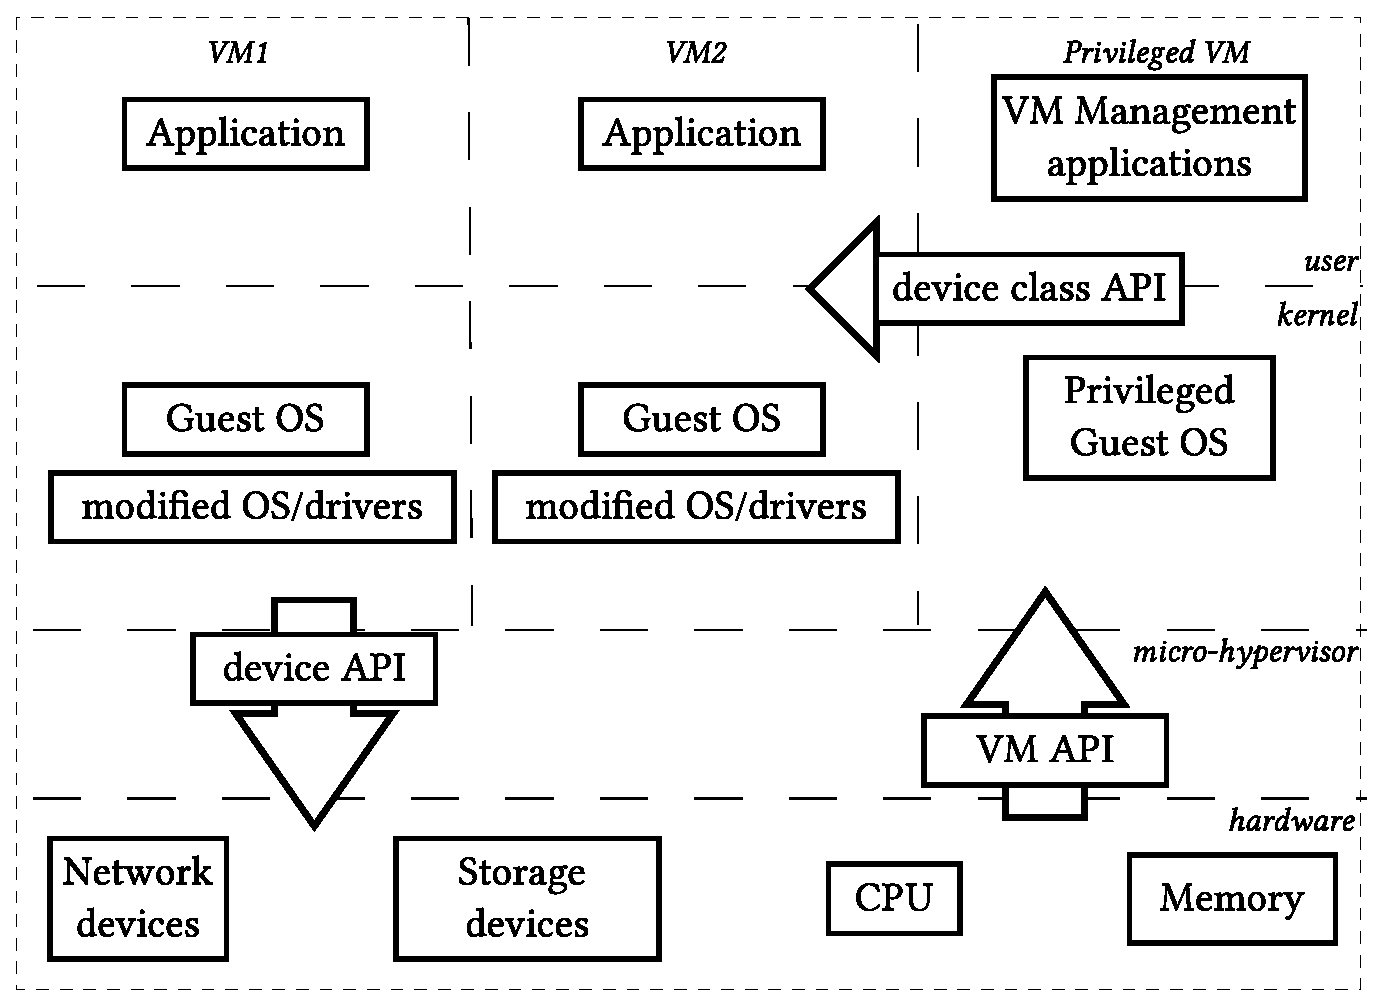
\includegraphics[width=.65\linewidth]{figures/paravirt.eps}
\end{figure}
\end{frame}

\section{I/O access in Virtualized Environments}

\subsection{Xen}
\begin{frame}
\frametitle{I/O Internals -- Xen}
\begin{block}{Xen basics}
                \begin{itemize}
                    \item hypervisor -- driver domain runs as a Linux guest
                    \item split driver model (frontend/backend)
                \end{itemize}
\end{block}
        \begin{block}{Xen -- Event channels}
                \begin{itemize}
                    \item notify Guest/Host about a pending transaction
                    \item easy to setup -- bind to a specific "port"
                \end{itemize}
        \end{block}
        \begin{block}{Xen -- Grant mechanism}
                \begin{itemize}
                    \item issue a page grant request
                    \item the other end maps the grant (accept)
                    \item this page is shared across the two domains
                \end{itemize}
        \end{block}

\end{frame}

\begin{frame}
\frametitle{I/O internals -- Xen Ring buffers}
\begin{columns}
\column{\textwidth}
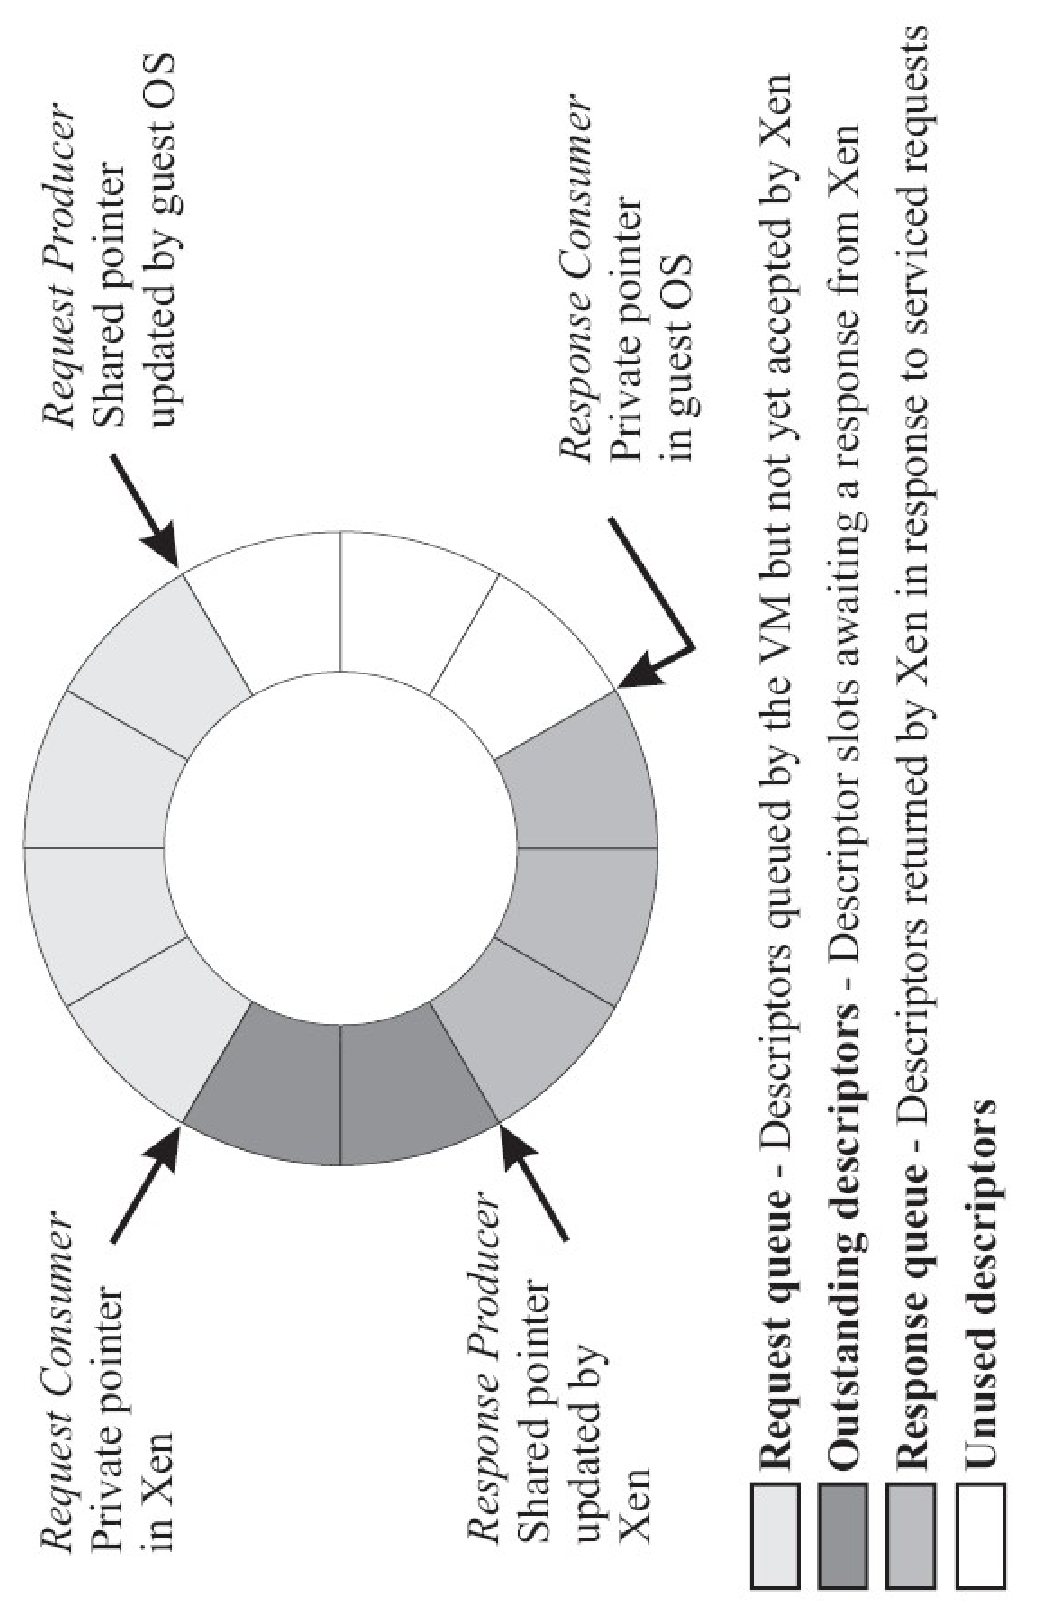
\includegraphics[width=.6\textwidth,angle=-90]{figures/test.eps}
\end{columns}
\end{frame}

%\begin{frame}
%\frametitle{Device Access - Split Driver Model}
%\begin{itemize}
%\item χρησιμοποιεί grant mechanism, event channels και ring buffers
%\item πραγματικός οδηγός
%\item κάτω μισό του διαχωρισμένου οδηγού (back-end)
%\item ring buffer
%\item πάνω μισό του διαχωρισμένου οδηγού (front-end)
%\end{itemize}
%%\begin{figure}
%%\includegraphics[scale=0.30]{figs/bare/io_paravirt.eps}
%%\end{figure}
%\end{frame}


\subsection{Intra-node communication in Xen}

\begin{frame}
\frametitle{I/O internals -- intra-node communication in Xen}
\begin{figure}
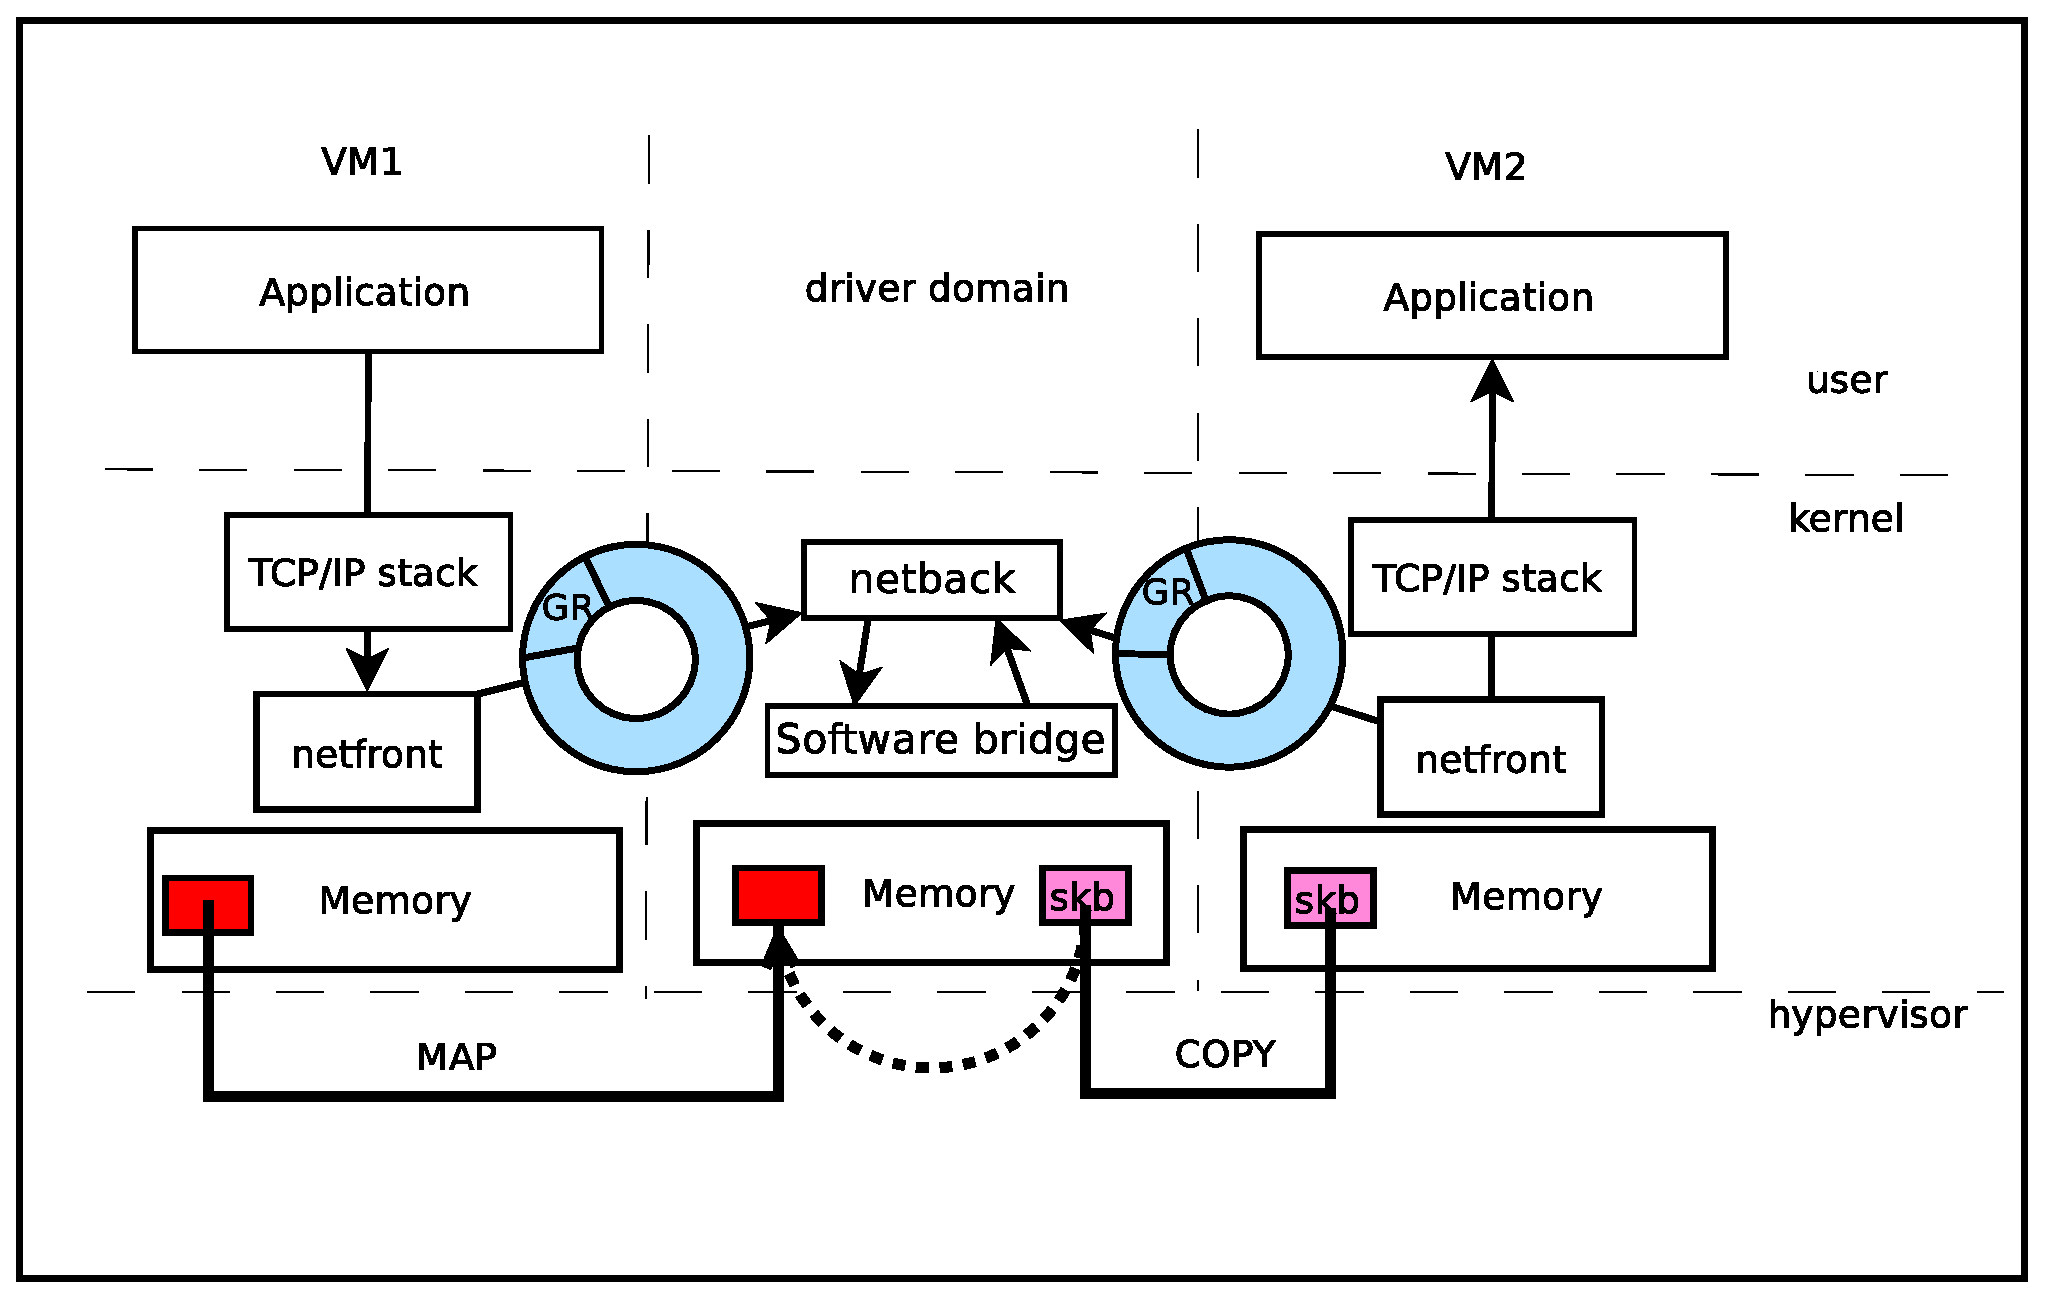
\includegraphics[width=.9\textwidth]{figures/netfront_netback.eps}
\end{figure}
\end{frame}


\section{V4VSockets}

\subsection{Architecture}

\begin{frame}
\frametitle{V4Vsockets vs Netfront/Netback}
\begin{figure}
\includegraphics[width=\textwidth]{figures/paths.eps}
\end{figure}
\end{frame}

\begin{frame}
\frametitle{V4VSockets Architecture}
\begin{columns}
\column{.8\textwidth}
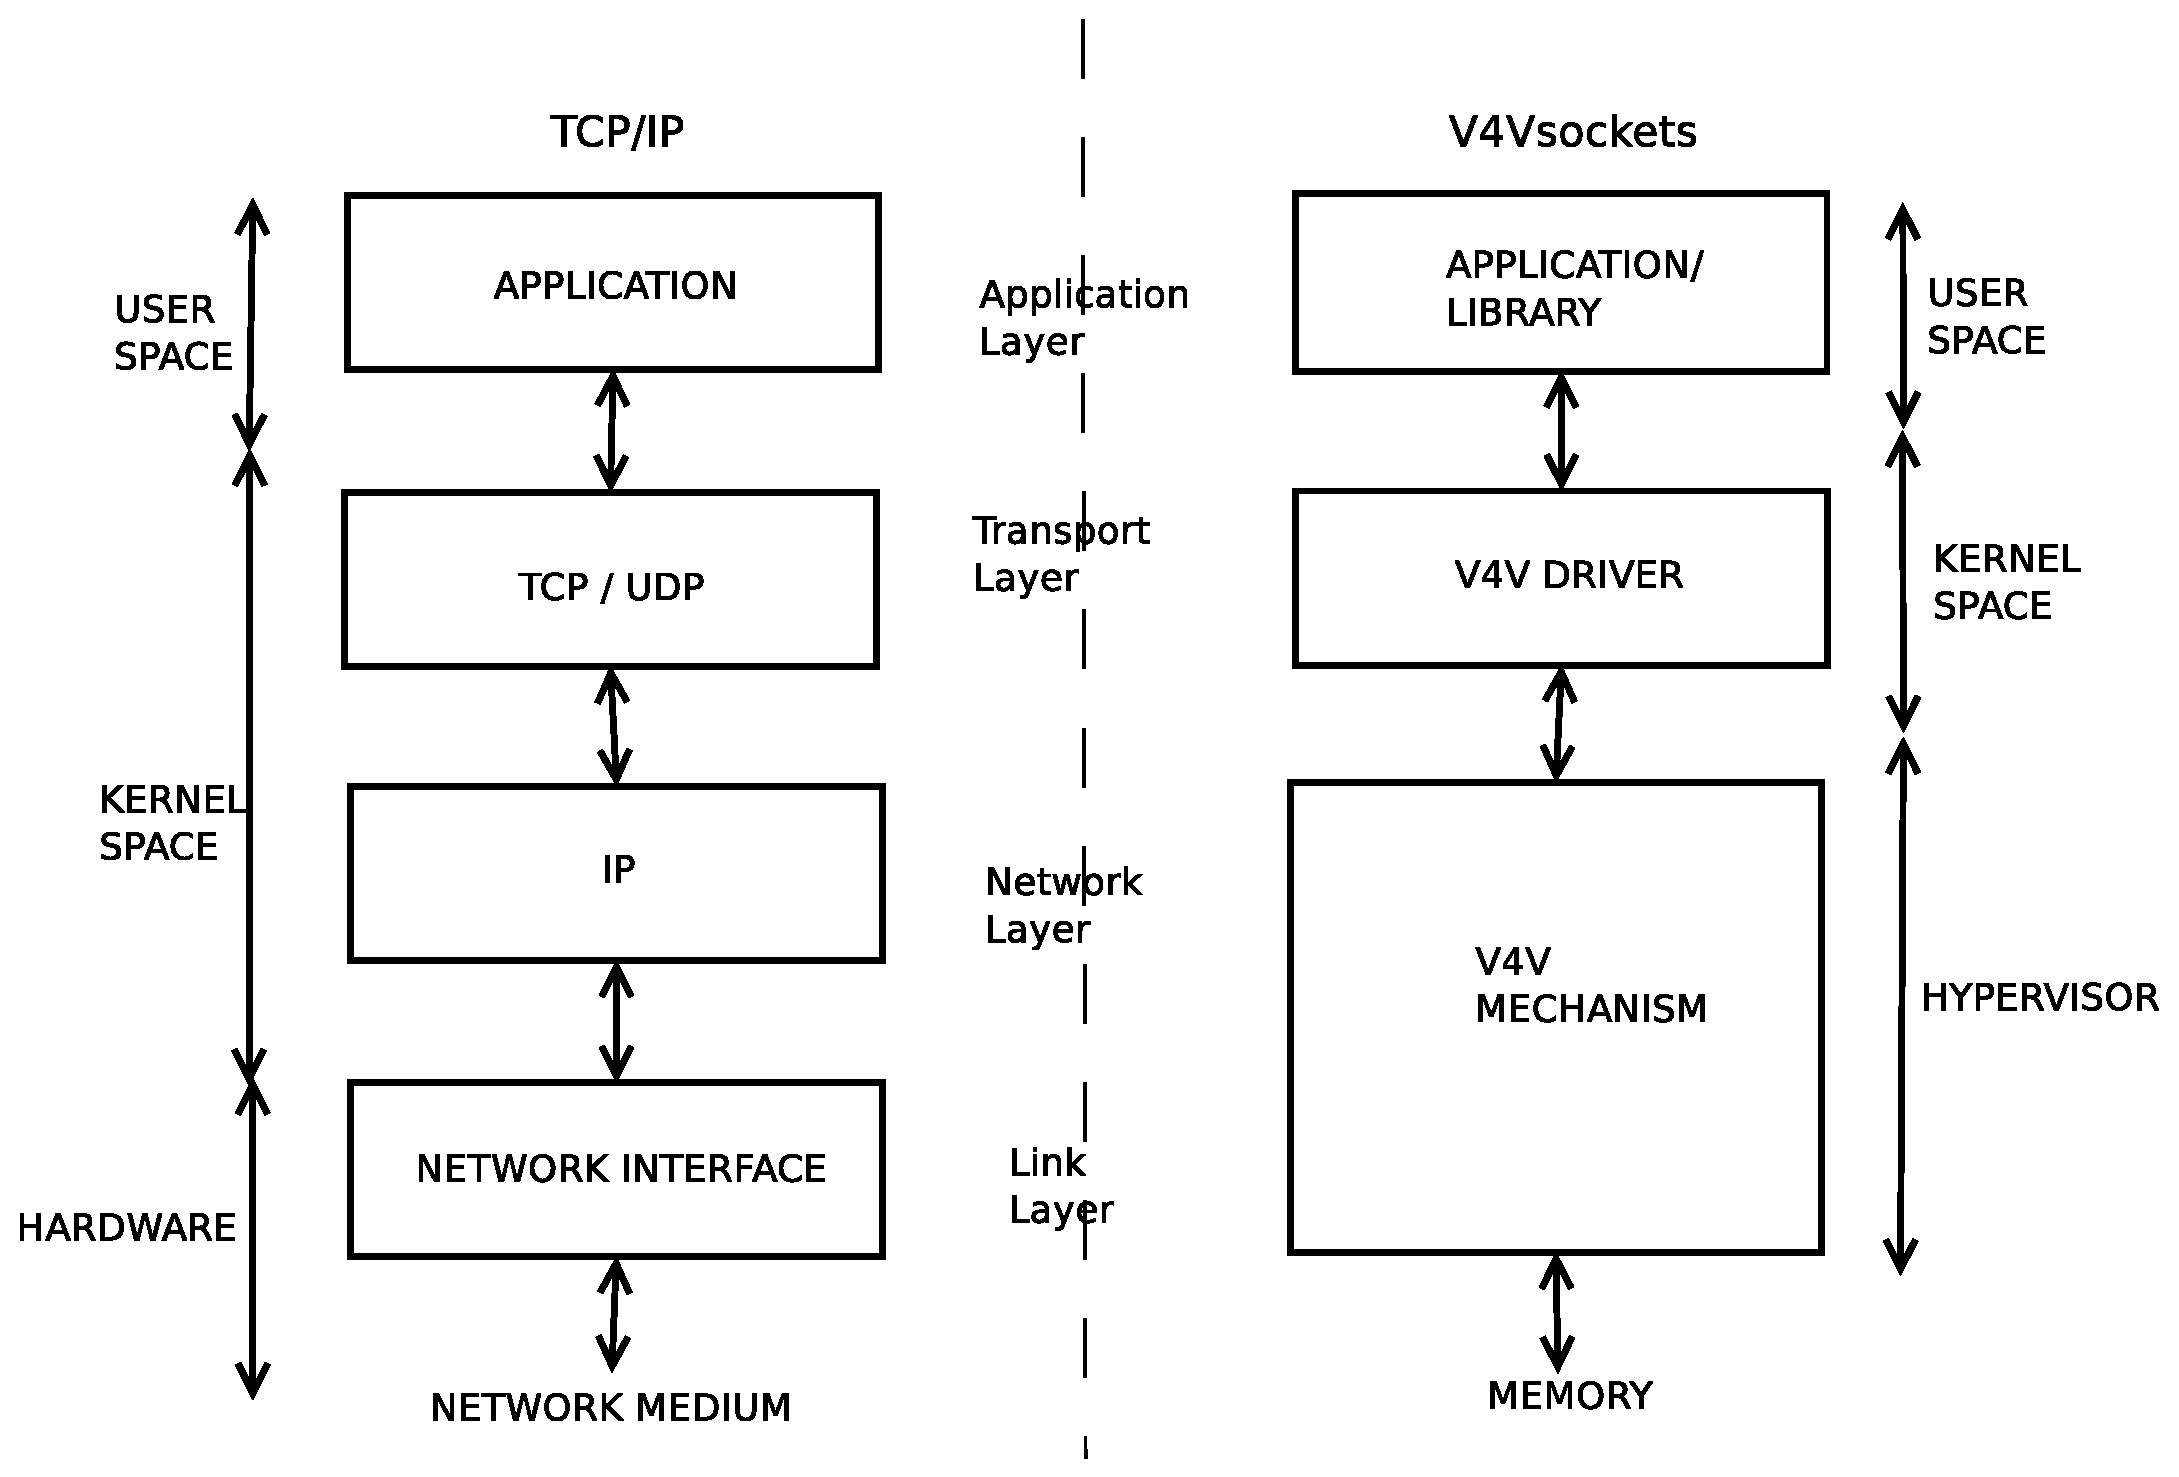
\includegraphics[width=\textwidth]{figures/tcp_ip_vs_v4vsockets.eps}
\end{columns}
\end{frame}

\begin{frame}
\frametitle{V4VSockets Internals}
\begin{block}{Communication mechanisms in V4VSockets}
\begin{itemize}
\item system calls 
\item hypercalls
\item event channels - VIRQS
\end{itemize}
\end{block}
\begin{block}{V4V Rings}
\begin{itemize}
\item circular buffers 
\item allocated in the VM address space by the VM kernel
\item data exchange medium
\end{itemize}
\end{block}
\end{frame}



\begin{frame}
\frametitle{V4VSockets Internals}
\begin{block}{Application/Library layer -- user--space}
\begin{itemize}
\item forwards the relevant actions and arguments to the transport layer.
\item kernel-level socket implementation for a new address family (\texttt{AF\_V4VSOCK})
\end{itemize}
\end{block}
\begin{block}{Example:}
\begin{itemize}
\item \texttt{socket()} $\rightarrow$ \texttt{v4vsockets\_create()}
\item \texttt{bind(sockaddr)} $\rightarrow$ \texttt{v4vsockets\_ring\_create(dom\_id, port)}
\item \texttt{sendmsg(msghdr)} $\rightarrow$ \texttt{v4vsockets\_sendmsg(msghdr)}
\end{itemize}
\end{block}
\end{frame}

\begin{frame}
\frametitle{V4VSockets Internals}
\begin{block}{Transport layer -- V4V frontend driver -- VM kernel}
\begin{itemize}
\item handles the virtual connection semantics between peer VMs that need to communicate,
\item is in charge of fragmenting and sending upper-layer packets by issuing hypercalls to the hypervisor (network layer), and
\item provides a notification mechanism to the VM's user-space for receiving packets, as well as error control.
\end{itemize}
\end{block}
\begin{block}{Example:}
\begin{itemize}
\item \texttt{v4vsockets\_sendmsg(msghdr)} $\rightarrow$ \\\texttt{while(nr\_iovecs) \\    v4v\_send(dom\_id, iovec)}
\end{itemize}
\end{block}
\end{frame}

\begin{frame}
\frametitle{V4VSockets Internals}
\begin{block}{Network/Link layer -- hypervisor}
\begin{itemize} 
\item encapsulation of upper-layer messages to packets that will be transmitted
to their destination, according to V4V semantics,
\item packet delivery.
\end{itemize}
\end{block}

\begin{block}{Example:}
\begin{itemize}
\item \texttt{v4v\_send(dom\_id, iovec)} $\rightarrow$ \\\texttt{dom\_ring = v4v\_resolve(dom\_id); \\memcpy(dom\_ring, iovec\_ptr, iovec\_len)}
\end{itemize}
\end{block}
\end{frame}


\begin{frame}
\frametitle{V4VSockets -- Message Exchange}
\begin{figure}
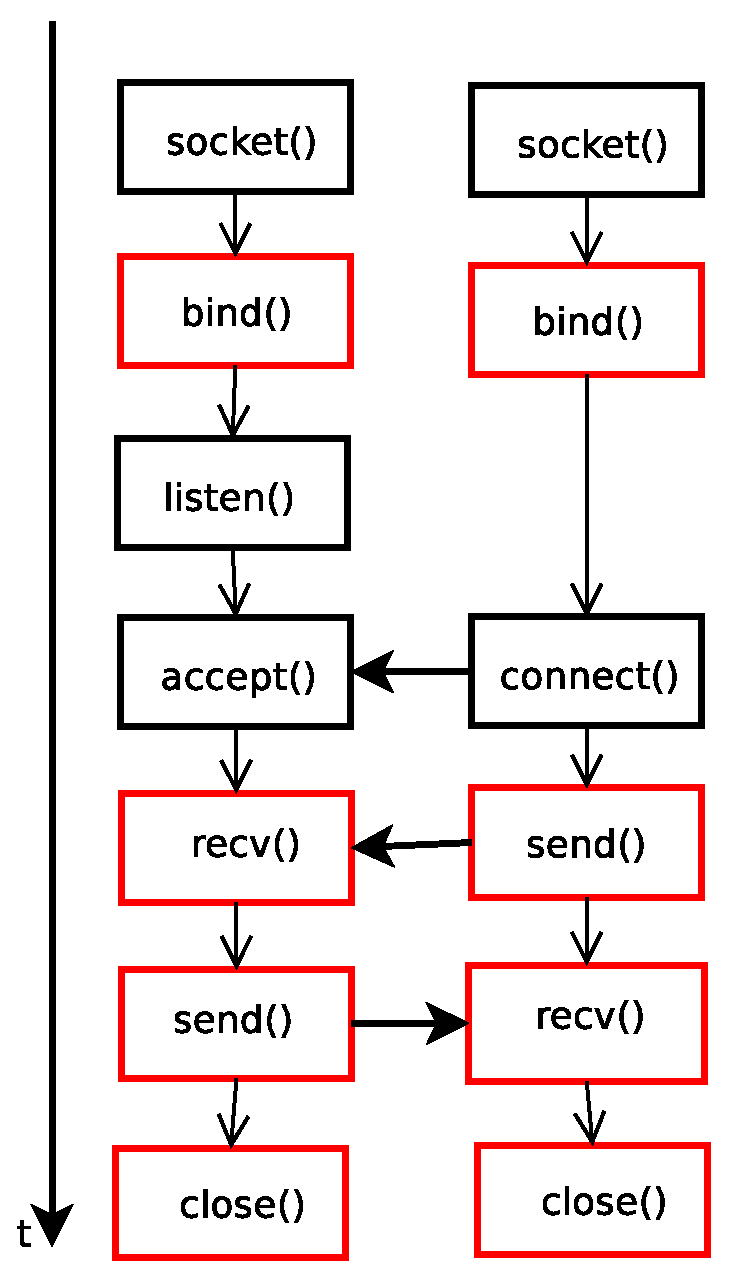
\includegraphics[scale=0.30]{figures/sockets.eps}
\end{figure}
\end{frame}

%\begin{frame}
%\frametitle{V4VSockets -- Message Exchange}
%\begin{figure}
%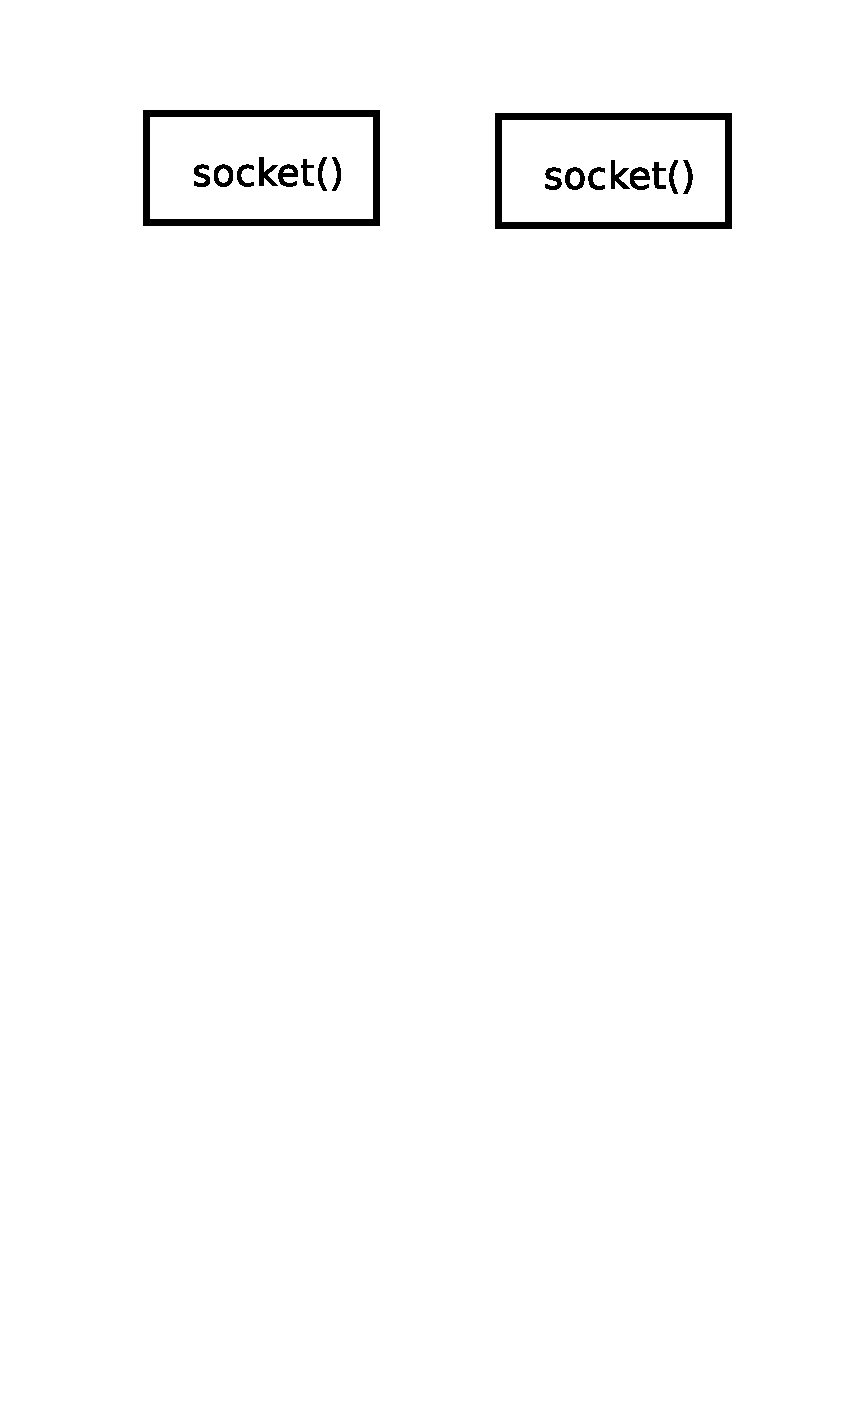
\includegraphics[scale=0.30]{figures/sockets6.eps}
%\end{figure}
%\end{frame}
%
%\begin{frame}
%\frametitle{V4VSockets -- Message Exchange}
%\begin{figure}
%\includegraphics[scale=0.30]{figures/sockets5.eps}
%\end{figure}
%\end{frame}
%
%\begin{frame}
%\frametitle{V4VSockets -- Message Exchange}
%\begin{figure}
%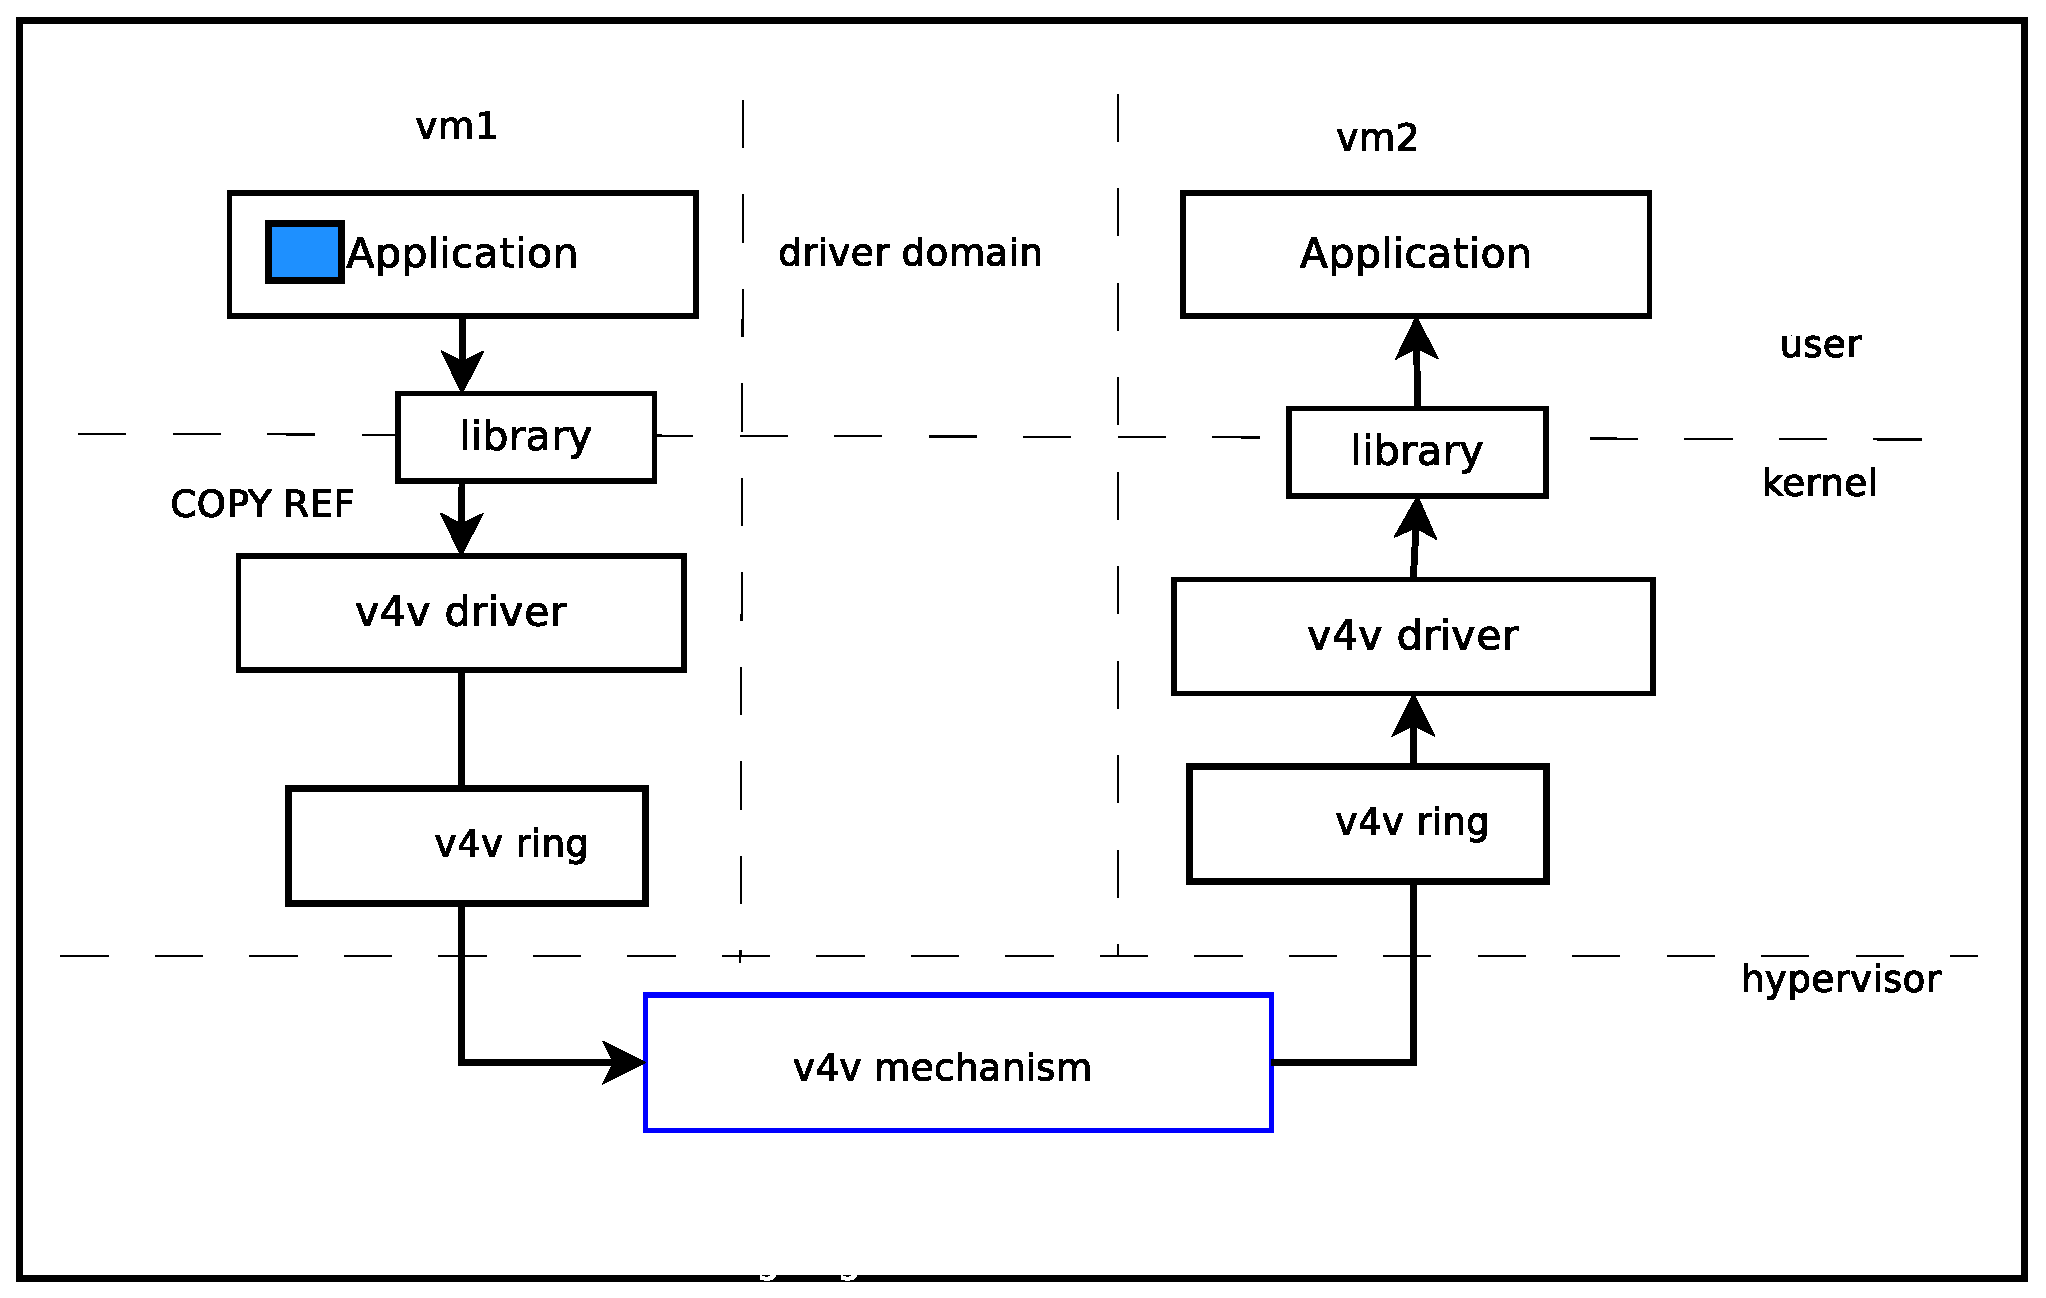
\includegraphics[scale=0.30]{figures/v4vsockets5.eps}
%\end{figure}
%\end{frame}
%
%\begin{frame}
%\frametitle{V4VSockets -- Message Exchange}
%\begin{figure}
%\includegraphics[scale=0.30]{figures/sockets4.eps}
%\end{figure}
%\end{frame}
%
%\begin{frame}
%\frametitle{V4VSockets -- Message Exchange}
%%\begin{columns}
%%\column{.8\textwidth}
%\begin{figure}
%\includegraphics[scale=0.30]{figures/sockets3.eps}
%\end{figure}
%\end{frame}
%
%\begin{frame}
%\frametitle{V4VSockets -- Message Exchange}
%\begin{figure}
%\includegraphics[scale=0.30]{figures/v4vsockets4.eps}
%\end{figure}
%\end{frame}
%
%\begin{frame}
%\frametitle{V4VSockets -- Message Exchange}
%\begin{figure}
%\includegraphics[scale=0.30]{figures/v4vsockets3.eps}
%\end{figure}
%\end{frame}
%
%
%\begin{frame}
%\frametitle{V4VSockets -- Message Exchange}
%%\begin{columns}
%%\column{.8\textwidth}
%\begin{figure}
%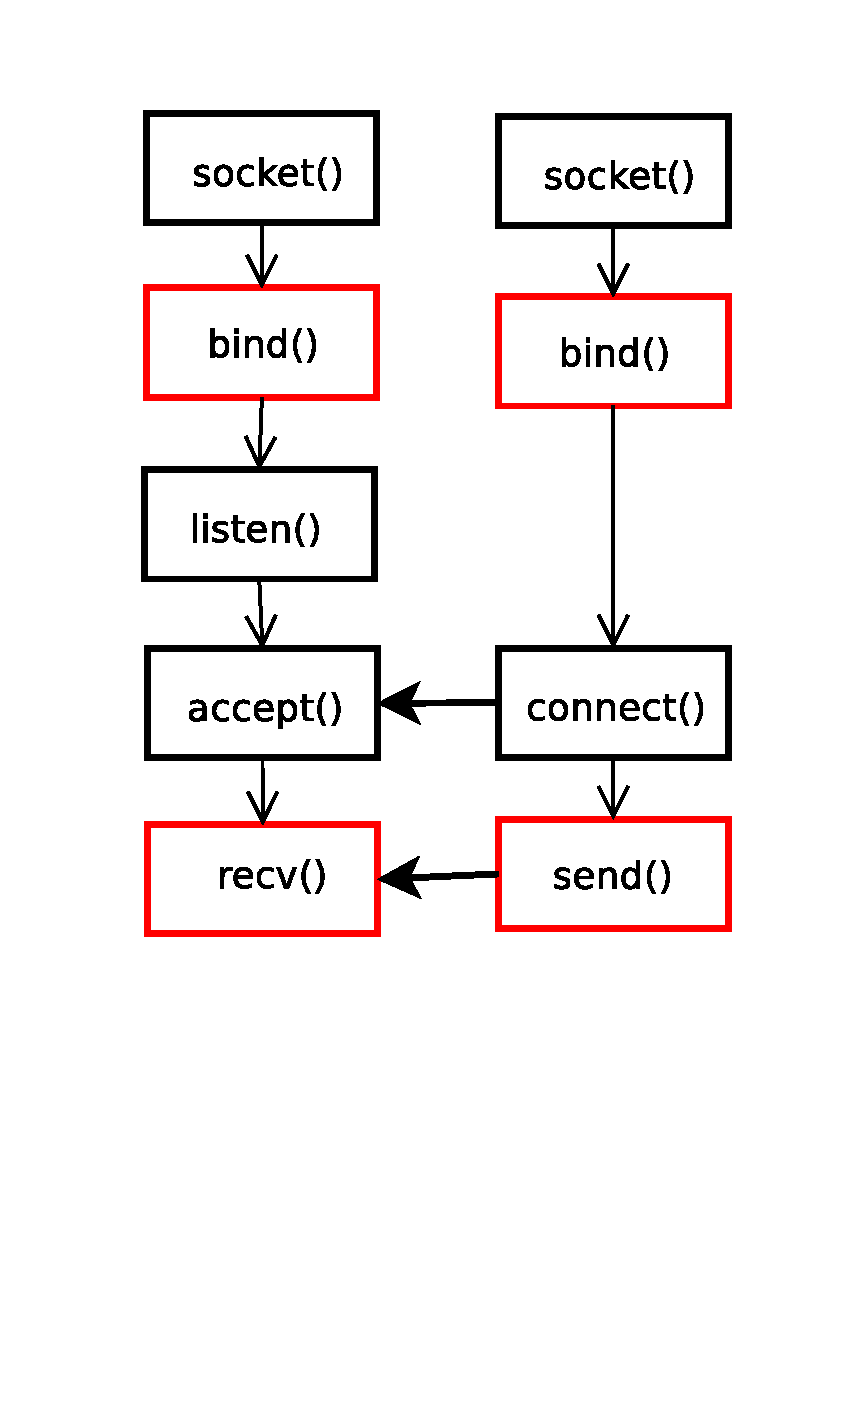
\includegraphics[scale=0.30]{figures/sockets2.eps}
%\end{figure}
%\end{frame}
%
%\begin{frame}
%\frametitle{V4VSockets -- Message Exchange}
%\begin{figure}
%\includegraphics[scale=0.30]{figures/v4vsockets2.eps}
%\end{figure}
%\end{frame}
%
%\begin{frame}
%\frametitle{V4VSockets -- Message Exchange}
%\begin{figure}
%\includegraphics[scale=0.30]{figures/v4vsockets1.eps}
%\end{figure}
%\end{frame}
%
\begin{frame}
\frametitle{V4VSockets -- Message Exchange}
\begin{figure}
\includegraphics[scale=0.30]{figures/v4vsockets.eps}
\end{figure}
\end{frame}



%\begin{frame}
%\frametitle{V4VSockets -- Message Exchange}
%\begin{figure}
%\includegraphics[scale=0.30]{figures/sockets1.eps}
%\end{figure}
%\end{frame}
%
%\begin{frame}
%\frametitle{V4VSockets -- Message Exchange}
%\begin{figure}
%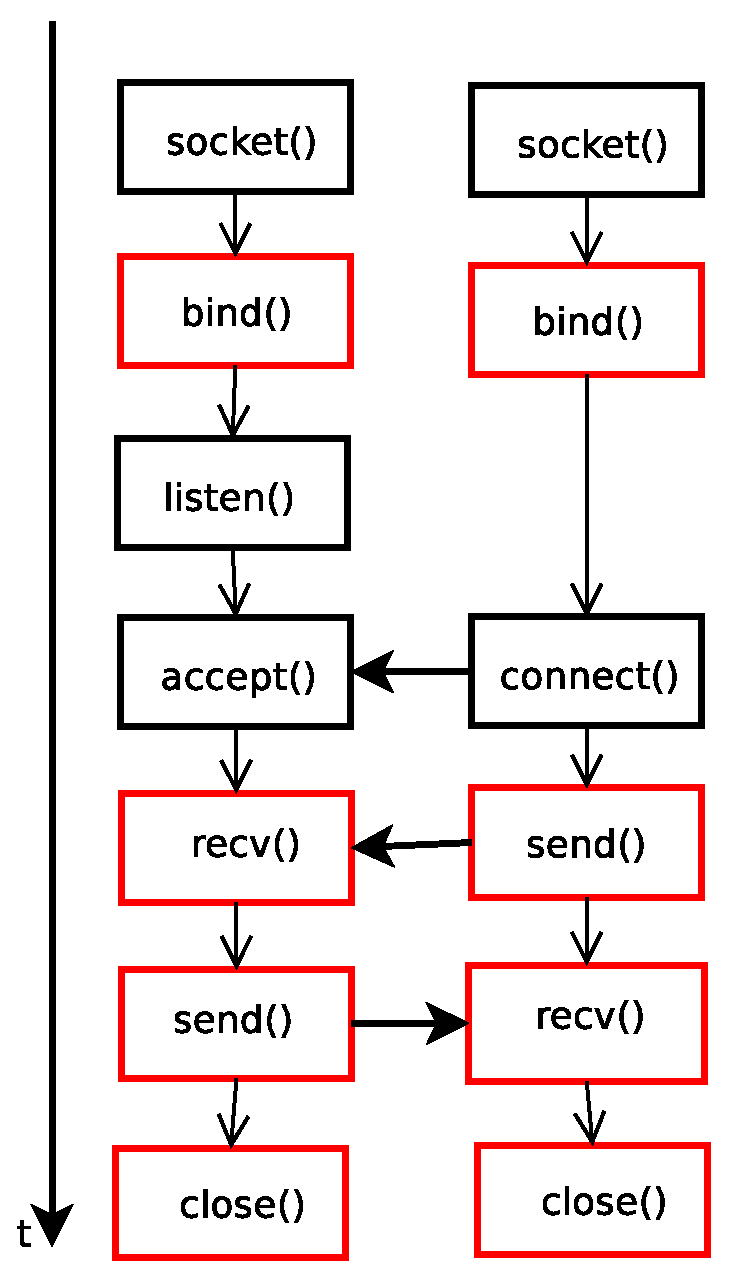
\includegraphics[scale=0.30]{figures/sockets.eps}
%\end{figure}
%\end{frame}
%
\subsection{Experimental Evaluation}

\begin{frame}
\frametitle{Experimental Evaluation}
\begin{block}{Testbed}
\begin{itemize}
\item 2x \{Intel Xeon @2.4Ghz\}, Intel 5520, 48GB memory
\item Xen 4.5-unstable, Debian GNU/Linux (Linux kernel 3.14.2)
\item generic micro-benchmark: \texttt{pingpong}
%\begin{itemize}
%\item[\tiny{$\leq$ 64b}]: copying
%\item[\tiny{$\leq$ 32KB}]: send \& receive queues
%\item[\tiny{$\geq$ 64KB}]: rendez-vous semantics
%\item$\leq$ 64b: αντιγραφή
%\item$\leq$ 32KB: ουρές αποστολής \& λήψης
%\item$\geq$ 64KB: σημασιολογία rendez-vous
%\end{itemize}
\end{itemize}
\end{block}
%\begin{block}
{Cases:}
\begin{itemize}
\item TCP sockets
\item V4V Stream
\end{itemize}
{Experiment setup:}
\begin{itemize}
\item 2 VMs exchanging messages (latency, throughput)
\item up to 16 VMs exchanging messages in pairs (latency, throughput)
\end{itemize}
%\end{block}
\end{frame}


\begin{frame}
\frametitle{Experimental evaluation -- latency}
\begin{columns}
\column{.8\textwidth}
\includegraphics[width=\textwidth]{figures/v4v_lat.eps}
\end{columns}
\end{frame}

\begin{frame}
\frametitle{Experimental evaluation -- throughput}
\begin{columns}
\column{.8\textwidth}
\includegraphics[width=\textwidth]{figures/v4v_bw.eps}
\end{columns}
\end{frame}

%\begin{frame}
%\frametitle{Πειραματική αποτίμηση -- μηνύματα 512K}
%\begin{columns}
%\column{.8\textwidth}
%\includegraphics[width=\textwidth]{figs/bare/aggregate_doms_cpu.eps}
%\end{columns}
%\end{frame}

\begin{frame}
\frametitle{Experimental evaluation -- latency scaling}
\begin{columns}
\column{.8\textwidth}
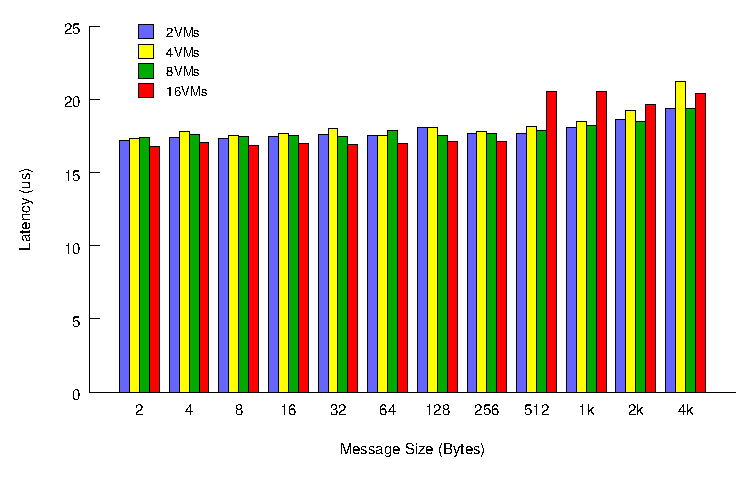
\includegraphics[width=\textwidth]{figures/lat_stream_scale.eps}
\end{columns}

\end{frame}
\begin{frame}
\frametitle{Experimental evaluation -- throughput scaling}
\begin{columns}
\column{.8\textwidth}
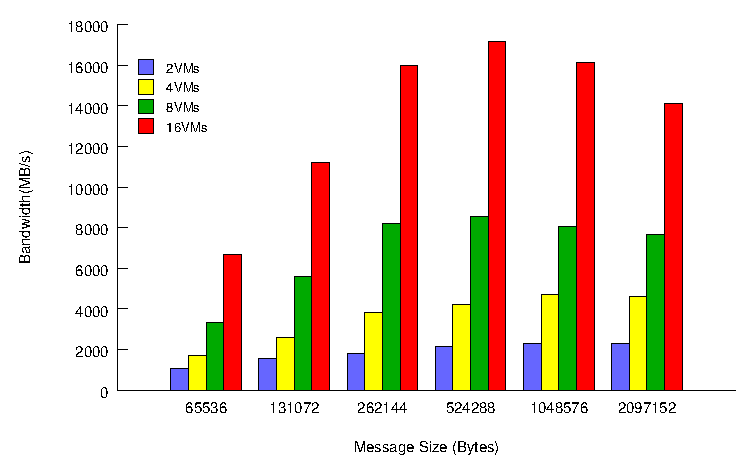
\includegraphics[width=\textwidth]{figures/bw_stream_scale.eps}
\end{columns}
\end{frame}

\begin{frame}

\frametitle{Experimental evaluation -- GPU stencil}
\begin{block}{Remote CUDA execution framework (rCUDA)}
\begin{itemize}
\item A.~J. Pe{\~{n}}a, C.~Rea{\~{n}}o, F.~Silla, R.~Mayo, E.~S.
  Quintana{-}Ort{\'{\i}}, and J.~Duato.
\emph{A complete and efficient cuda-sharing solution for {HPC} clusters}.
\emph{Parallel Computing}, 40\penalty0 (10):\penalty0 574--588, 2014.
\item execute remote CUDA calls through TCP sockets
\item direct assignment (PCI passthrough)
\item remote calls via TCP sockets and V4VSockets
\end{itemize}
\end{block}

\begin{block}{GPU stencil: matrix-matrix product benchmark}
\begin{itemize}
\item plot total time of execution
\item plot transfer time of first input matrix
\end{itemize}
\end{block}
\end{frame}


\begin{frame}
\frametitle{Experimental evaluation -- GPU stencil}
\begin{columns}
\column{.8\textwidth}
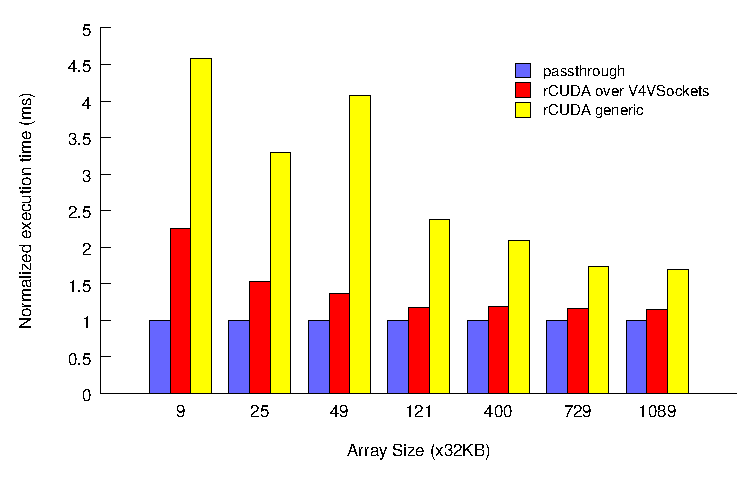
\includegraphics[width=\textwidth]{figures/total_cublas_time.eps}
\end{columns}
\end{frame}

\begin{frame}
\frametitle{Experimental evaluation -- GPU stencil}
\begin{columns}
\column{.8\textwidth}
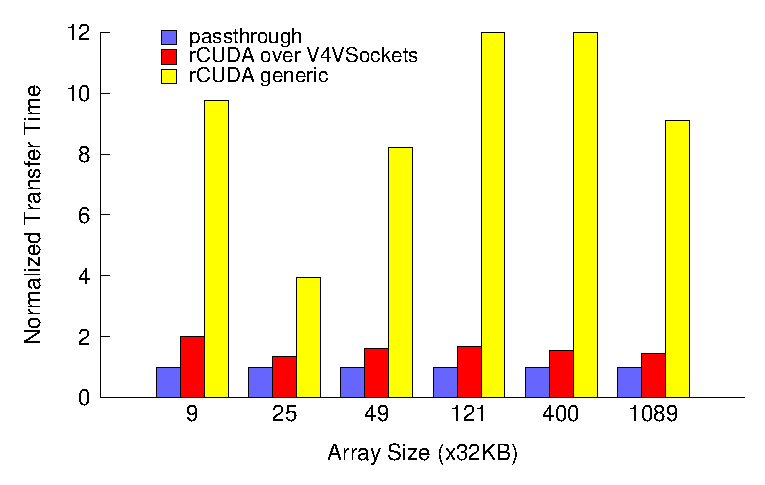
\includegraphics[width=\textwidth]{figures/matrixA_cublas_throughput.eps}
\end{columns}
\end{frame}

\section*{Conclusions}

\subsection*{Summary}

\begin{frame}
\frametitle{Summary}
\begin{block}{Intra-node communication in VM environments}
\begin{itemize}
\item split driver model -- generic
\item V4VSockets: framework for low-overhead intra-node communication
\begin{itemize}
\item is not based on a driver domain
\item does not use shared memory between guests (map/grant mechanism)
\item uses memory copies, hypercalls and event channels
%πρωτόκολλο διασύνδεσης σχεδιασμένο για εικονικά περιβάλλοντα
\end{itemize}
\end{itemize}
\end{block}
%\begin{block}{V4VSockets}
\begin{itemize}
\item better throughput (efficient data path, bypass the complex TCP/IP stack)
\item hypercall overheads (small, negligible if correctly finetuned)
\item scalability (no privileged guest involved in communication)
\item isolation (no shared memory)
\item event driven%(layered design, χωρισμένο σε link layer και protocol layer).
%\item hypervisor-specific transport layer, generic interface
%πρωτόκολλο διασύνδεσης σχεδιασμένο για εικονικά περιβάλλοντα
\end{itemize}
%\end{block}
\end{frame}

\begin{frame}
\frametitle{Future endaevors}
\begin{itemize}
%\item ένταξη σημασιολογίας δικτύων υψηλής επίδοσης στο μοντέλο διαχωρισμένου οδηγού
%\item επικοινωνία με πολύ χαμηλό χρόνο απόκρισης και υψηλή ρυθμαπόδοση -- συγκρίσιμα με περιβάλλοντα χωρίς virtualization
%\item συμβατότητα με πρωτόκολλα ανώτερων στρωμάτων (MPI κλπ.)
\item CPU utilization overheads
\item NUMA and multihierarchical memory architectures
\item map instead of copy (study the systems behavior of providing a shared memory space between VMs)
\item GPU sharing evaluation
\end{itemize}
%\begin{block}{Future Plans:}
%\begin{itemize}
%\item optimize Xen2MX to reach native performance numbers
%\item generalize the case to different hypervisors
%\end{itemize}
%\end{block}

Available online as open-source \url{https://github.com/HPSI/V4VSockets}

\end{frame}
%
\begin{frame}
\frametitle{Thanks!}
                \vfill%
\begin{columns}
        \column{.35\textwidth}
        \begin{center}
                %\vfill%
            %    \begin{block}{}
        \begin{center}
                        {\LARGE Questions?}
        \end{center}
             %   \end{block}
                \vfill%
                %\vfill%
        \end{center}
\end{columns}
                \vfill%
\end{frame}


\begin{frame}
\frametitle{}
                \vfill%
\begin{columns}
        \column{.35\textwidth}
        \begin{center}
                %\vfill%
            %    \begin{block}{}
             %   \end{block}
                \vfill%
                %\vfill%
        \end{center}
\end{columns}
                \vfill%
\end{frame}
%
\begin{frame}
\frametitle{}
                \vfill%
\begin{columns}
        \column{.35\textwidth}
        \begin{center}
                %\vfill%
            %    \begin{block}{}
        \begin{center}
                        {\LARGE Backup}
        \end{center}
             %   \end{block}
                \vfill%
                %\vfill%
        \end{center}
\end{columns}
                \vfill%
\end{frame}

\begin{frame}
\frametitle{Experimental evaluation -- 2M message size vs Hypercalls}
\begin{columns}
\column{.8\textwidth}
\includegraphics[width=\textwidth]{figures/2M.eps}
\end{columns}
\end{frame}

\begin{frame}
\frametitle{Experimental evaluation -- Datagram scalability}
\begin{columns}
\column{.8\textwidth}
\includegraphics[width=\textwidth]{figures/bw_dgram_scale.eps}
\end{columns}
\end{frame}

\begin{frame}
\frametitle{Experimental evaluation -- Hypercalls per message}
\begin{columns}
\column{.8\textwidth}
\includegraphics[width=\textwidth]{figures/mix.eps}
\end{columns}
\end{frame}
%
%\begin{frame}
%\frametitle{Πειραματική αποτίμηση -- Ποσοστό χρήσης CPU για το VM}
%\begin{columns}
%\column{.8\textwidth}
%\includegraphics[width=\textwidth]{figs/bare/lat_breakdown_domU.eps}
%\end{columns}
%\end{frame}
%
%\begin{frame}
%\frametitle{Xen2MX -- I}
%\begin{columns}
%\column{.8\textwidth}
%\includegraphics[width=\textwidth]{figs/bare/xen2mx_step1.pdf}
%\end{columns}
%\end{frame}
%
%\begin{frame}
%\frametitle{Xen2MX -- II}
%\begin{columns}
%\column{.8\textwidth}
%\includegraphics[width=\textwidth]{figs/bare/xen2mx_step2.pdf}
%\end{columns}
%\end{frame}
%
%\begin{frame}
%\frametitle{Xen2MX -- III}
%\begin{columns}
%\column{.8\textwidth}
%\includegraphics[width=\textwidth]{figs/bare/xen2mx_step3.pdf}
%\end{columns}
%\end{frame}
%
%\begin{frame}
%\frametitle{Xen2MX -- IV (Bridged)}
%\begin{columns}
%\column{.8\textwidth}
%\includegraphics[width=\textwidth]{figs/bare/xen2mx_step4.pdf}
%\end{columns}
%\end{frame}
%
%\begin{frame}
%\frametitle{Xen2MX -- ΙV (IOV)}
%\begin{columns}
%\column{.8\textwidth}
%\includegraphics[width=\textwidth]{figs/bare/xen2mx_step5.pdf}
%\end{columns}
%\end{frame}
%
%\begin{frame}
%\frametitle{Xen2MX -- IV (Xen2MX)}
%\begin{columns}
%\column{.8\textwidth}
%\includegraphics[width=\textwidth]{figs/bare/xen2mx_step6.pdf}
%\end{columns}
%\end{frame}
%

\begin{thebibliography}{14}
%\providecommand{\natexlab}[1]{#1}
%\providecommand{\url}[1]{\texttt{#1}}
%\expandafter\ifx\csname urlstyle\endcsname\relax
%  \providecommand{\doi}[1]{doi: #1}\else
%  \providecommand{\doi}{doi: \begingroup \urlstyle{rm}\Url}\fi
%
%\bibitem[Barham et~al.(2003)Barham, Dragovic, Fraser, Hand, Harris, Ho,
%  Neugebauer, Pratt, and Warfield]{barham03sosp}
%P.~Barham, B.~Dragovic, K.~Fraser, S.~Hand, T.~Harris, A.~Ho, R.~Neugebauer,
%  I.~A. Pratt, and A.~Warfield.
%\newblock Xen and the art of virtualization.
%\newblock In \emph{SOSP '03: Proc. of the 19th ACM symposium on Operating
%  systems principles}, pages 164--177, New York, NY, USA, 2003. ACM.
%
%\bibitem[Huang et~al.(2007)Huang, Koop, Gao, and Panda]{huang07mpivm}
%W.~Huang, M.~J. Koop, Q.~Gao, and D.~K. Panda.
%\newblock {Virtual machine aware communication libraries for high performance
%  computing}.
%\newblock In \emph{SC '07: Proceedings of the 2007 ACM/IEEE conference on
%  Supercomputing}, NY, USA, 2007. ACM.
%\newblock ISBN 978-1-59593-764-3.
%\newblock \doi{10.1145/1362622.1362635}.
%
%\bibitem[Kim et~al.(2008)Kim, Kim, Jung, Shin, and Kim]{kim2008sockets}
%K.~Kim, C.-Y. Kim, S.-I. Jung, H.-S. Shin, and J.-S. Kim.
%\newblock Inter-domain socket communications supporting high performance and
%  full binary compatibility on xen.
%\newblock In \emph{Proceedings of the Fourth ACM SIGPLAN/SIGOPS International
%  Conference on Virtual Execution Environments}, VEE '08, pages 11--20, New
%  York, NY, USA, 2008. ACM.
%\newblock ISBN 978-1-59593-796-4.
%\newblock \doi{10.1145/1346256.1346259}.
%
%\bibitem[Menon et~al.(2006)Menon, Cox, and Zwaenepoel]{menon06atec}
%A.~Menon, A.~L. Cox, and W.~Zwaenepoel.
%\newblock {Optimizing network virtualization in Xen}.
%\newblock In \emph{ATEC '06: Proceedings of the annual conference on USENIX '06
%  Annual Technical Conference}, pages 2--2, Berkeley, CA, USA, 2006. USENIX.
%
%\bibitem[Nanos et~al.(2010)Nanos, Goumas, and Koziris]{nanos10vhpc}
%A.~Nanos, G.~Goumas, and N.~Koziris.
%\newblock Exploring {I/O} virtualization data paths for {MPI} applications in a
%  cluster of {VMs:} a networking perspective.
%\newblock In \emph{5th Workshop on Virtualization in High-Performance Cloud
%  Computing (VHPC '10)}, Ischia - Naples, Italy, 8 2010.
%
%\bibitem[NetPIPE - Network Protocol Independent Performance
%  Evaluator()]{netpipe}
%NetPIPE - Network Protocol Independent Performance Evaluator.
%\newblock {\url{http://linux.die.net/man/1/netpipe}}.
%
%\bibitem[NVIDIA CUDA samples()]{cudasamples}
%NVIDIA CUDA samples.
%\newblock {\url{https://developer.nvidia.com/cuda-downloads}}.
%
%\bibitem[Pe{\~{n}}a et~al.(2014)Pe{\~{n}}a, Rea{\~{n}}o, Silla, Mayo,
%  Quintana{-}Ort{\'{\i}}, and Duato]{rCUDAPena}
%A.~J. Pe{\~{n}}a, C.~Rea{\~{n}}o, F.~Silla, R.~Mayo, E.~S.
%  Quintana{-}Ort{\'{\i}}, and J.~Duato.
%\newblock A complete and efficient cuda-sharing solution for {HPC} clusters.
%\newblock \emph{Parallel Computing}, 40\penalty0 (10):\penalty0 574--588, 2014.
%
%\bibitem[Radhakrishnan and Srinivasan(2008)]{prashanth08mmnet}
%P.~Radhakrishnan and K.~Srinivasan.
%\newblock Mmnet: An efficient inter-vm communication mechanism.
%\newblock In \emph{XenSummit}, 2008.
%
%\bibitem[Santos et~al.(2008)Santos, Turner, Janakiraman, and
%  Pratt]{santos08atc}
%J.~R. Santos, Y.~Turner, G.~Janakiraman, and I.~Pratt.
%\newblock {Bridging the gap between software and hardware techniques for I/O
%  virtualization}.
%\newblock In \emph{ATC'08: USENIX 2008 Annual Technical Conference on Annual
%  Technical Conference}, pages 29--42, Berkeley, CA, USA, 2008. USENIX.
%
%\bibitem[V4V implementation()]{v4v2013}
%V4V implementation.
%\newblock
%  {\url{http://lists.xen.org/archives/html/xen-devel/2013-05/msg02711.html}}.
%
%\bibitem[Wang et~al.(2008)Wang, Wright, and Gopalan]{wang08hpdc}
%J.~Wang, K.-L. Wright, and K.~Gopalan.
%\newblock {XenLoop: a transparent high performance inter-vm network loopback}.
%\newblock In \emph{HPDC '08: Proceedings of the 17th international symposium on
%  High performance distributed computing}, pages 109--118, NY, USA, 2008. ACM.
%\newblock ISBN 978-1-59593-997-5.
%\newblock \doi{10.1145/1383422.1383437}.
%
%\bibitem[Youseff et~al.(2006)Youseff, Wolski, Gorda, and
%  Krintz]{youseff06paravirt}
%L.~Youseff, R.~Wolski, B.~Gorda, and R.~Krintz.
%\newblock {Paravirtualization for HPC Systems}.
%\newblock In \emph{In Proc. Workshop on Xen in High-Performance Cluster and
%  Grid Computing}, pages 474--486. Springer, 2006.
%
%\bibitem[Zhang et~al.(2007)Zhang, McIntosh, Rohatgi, and
%  Griffin]{zhang07xensocket}
%X.~Zhang, S.~McIntosh, P.~Rohatgi, and J.~Griffin.
%\newblock Xensocket: A high-throughput interdomain transport for virtual
%  machines.
%\newblock In R.~Cerqueira and R.~Campbell, editors, \emph{Middleware 2007},
%  Lecture Notes in Computer Science. 2007.
%
\end{thebibliography}

\end{document}
